\begin{introduction}
    \item 有界线性算子~\ref{BX}
    \item $Banach$-$Steinhaus$定理~\ref{BS}
    \item 开映射定理与闭图像定理~\ref{kb}
\end{introduction}
\section{有界线性算子}\label{BX}
在正式介绍赋范线性空间的有界线性算子之前,我们可以回忆一下有限维的情形,设$X,Y$为有限维空间,根据上一小节的描述,我们不妨假设$X=\mathbb{R}^m,Y=\mathbb{R}^n$,考虑线性变换$L:\mathbb{R}^m \to \mathbb{R}^n$,选取基底$\{e_i\}_{i=1}^m \subset X , \{f_j\}_{j=1}^n \subset Y$,线性变换$L$在基底上有如下关系
\[Le_i=\sum_j^na_{ij}f_j \ (a_{ij} \in \mathbb{R})\]
则$L$等价于矩阵$A=(a_{ij})_{1 \leq i \leq m , 1 \leq j \leq n}$,取
\[x=\sum_{i=1}^m\xi_ie_i \in X \ , \ y=\sum_{j=1}^n\eta_jf_j \quad \text{则} \quad Lx=
\begin{pmatrix}
    a_{11} & a_{12} & \cdots & a_{1m} \\
    a_{21} & a_{22} & \cdots & a_{2m} \\
    \vdots & \vdots & \ddots & \vdots \\
    a_{n1} & a_{n2} & \cdots & a_{nm} \\
\end{pmatrix}
\begin{pmatrix}
    \xi_1 \\ \xi_2 \\ \vdots \\ \xi_m \\
\end{pmatrix}
=\begin{pmatrix}
    \eta_1 \\ \eta_2 \\ \vdots \\ \eta_n \\
\end{pmatrix}
=y
\]

众所周知,泛函分析至少无穷维的线性代数,所以类似的我们可以延拓线性变换的定义到线性算子。
\begin{definition}[线性算子]
    设$X,Y$是赋范线性空间,$T$是从$X$的线性子空间$D(T) \subset X$到$Y$的映射,若其满足
    \[\forall x,y \in X \ , \ \alpha,\beta \in \mathbb{K} \ , \ T(\alpha x+\beta y)=\alpha Tx+\beta Ty\]
\end{definition}
值得注意的是线性算子的定义并不要求其定义域是出发空间的全空间,只要求是出发空间的一个线性子空间即可,当然可以是平凡子空间$(D(T)=X)$,但是默认全空间更省事所以一般默认全空间,同时无穷维的子空间也可以是稠密的$(C[0,1] \subset L[0,1])$。

回应一下章节标题,现在该定义线性算子的有界。
\begin{definition}[有界线性算子]
    设$T:X \to Y$是线性算子,若其满足
    \[\exists \, M>0 \quad \text{s.t.} \quad ||Tx||_Y \leq M||x||_x \ (\forall x \in X)\]
    则称其为有界线性算子。
\end{definition}
从$X \to Y$的全体有界线性算子记为$\mathscr{B}(X,Y)$。有界线性算子具有一些不错的性质,可以看下面一个定理。
\begin{theorem}
    设$T:X \to Y$是线性算子,则:\\
    1、$T$连续等价于$T$在一点处连续;\\
    2、$T$连续等价于$T$有界。
\end{theorem}
\textbf{Proof} of (1):“$\Rightarrow$” 显然

“$\Leftarrow$” 设$T$在$x_0 \in X$连续$\quad \Leftrightarrow \quad x_n \to x \ \Rightarrow \ Tx_n \to Tx$,则有
\[Tx_n-Tx=T(x_n-x+y)-Ty \to 0 \quad (\forall y \in X)\]

\textbf{Proof} of (2):“$\Leftarrow$” 由(1)知只需证明在一点处连续,不妨取为原点,取收敛于原点的点列$\{x_n\}$,由有界性
\[||Tx_n|| \leq M||x_n|| \to 0 \quad \Rightarrow \quad Tx_n \to 0 \quad \Leftrightarrow \quad Tx_n-T0 \to 0 \ (x_n-0 \to 0)\]

“$\Rightarrow$” 反证,设$T$连续但是无界,$\forall n \in \mathbb{N} \ , \ \exists \, x_n \in X \quad \text{s.t.} \quad ||Tx_n||>n||x_n||$,令
\[y_n=\frac{x_n}{n||x_n||} \ , \ ||y_n||=\frac{||x_n||}{n||x_n||}=\frac{1}{n} \to 0 \quad \Rightarrow \quad y_n \to 0\]

由线性性可知$T0=0$,而
\[||Ty_n-T0||=||Ty_n||=\left\|\frac{Tx_n}{n||x_n||}\right\|>1\]

与连续性矛盾。

\textbf{Q.E.D.}

上面提到了算子的有界性,那么自然外面会想用一个指标来衡量一个算子到底多有界,于是就有了算子范数的概念。
\begin{definition}[算子范数]
    设$T \in \mathscr{B}(X,Y)$,定义算子范数
    \[||T||=\mathop \text{sup}\limits_{x \in X/\{0\}}\frac{||Tx||}{||x||}=\mathop \text{sup}\limits_{||x||=1}||Tx||=\mathop \text{sup}\limits_{||x|| \leq 1}||Tx||\]
\end{definition}
既然叫范数说明$||T||$满足范数要求的条件这里不过多赘述,同时上述三个定义也是等价的,这些内容留待读者自证(笑

因此$(\mathscr{B}(X,Y),||\cdot||)$就构成了一个赋范线性空间,这还是比较有意思的,当然后面会更有意思(笑

另外一件事关于之前提到的线性算子的定义域的内容,我们说线性算子的定义域可以是出发空间的一个子空间也可以是出发空间本身,这两者在叫法上就区分为:
1、$T:D(T)=X \to Y$在$X$上到$Y$上;2、$T:D(T) \subset X \to Y$在$X$中到$Y$上。

下面我们来看几个例子。
\paragraph*{例1} \quad $X=\mathbb{R}^m,Y=\mathbb{R}^n \ , \ L \in \mathscr{B}(X,Y)$,选定基底后$L$等价于矩阵$A=(a_{ij})_{m \times n}$,分别取$X,Y$空间中的两个元素,$x,y$满足
\[x=(\xi_1,\xi_2,\cdots,\xi_m)^{\text{T}} \ , \ y=(\eta_1,\eta_2,\cdots,\eta_n)^{\text{T}} \ , \ Lx=y\]
则
\[||Lx||=||y||=\sqrt{\sum_{i=1}^n|\eta_i|^2}=\sqrt{\sum_{i=1}^n\left|\sum_{j=1}^ma_{ij}\xi_j\right|^2} \leq \sqrt{\sum_{i=1}^n\sum_{j=1}^ma_{ij}^2 \cdot \sum_{j=1}^m\xi_j^2}=\text{tr}(A^{\text{T}}A)^{\frac{1}{2}}||x||:=||A||\cdot||X||\]
由上确界性质可知$||L|| \leq ||A||$,实际上是取等。

\paragraph*{例2} \quad 微分算子,一维情形下,考虑$X=C[0,1] \ , \ T:X \to X \ , \ x(t) \mapsto Tx=x'(t)$,则该算子为无解算子:
\[x_n(t)=\sin nt \ , \ ||x_n||=1 \quad \Rightarrow \quad Tx_n=x_n'(t)=n \cos nt \ , \ ||Tx_n||=n \to +\infty\]

高维情形下也类似,考虑$\Omega \subset \mathbb{R}^n$,记$C^k(\bar{\Omega})=\{f:\bar{\Omega} \to \mathbb{R}|\partial^{\alpha}f \in C(\bar{\Omega}) \ , \ |\alpha| \leq k\}$,其上范数为:
\[||f||_{C^k}=\mathop \text{max}\limits_{|\alpha| \leq k}||\partial^{\alpha}f||_{C^0}=\mathop \text{max}\limits_{|\alpha| \leq k}\mathop \text{max}\limits_{x \in \bar{\Omega}}|\partial^{\alpha}f(x)|\]
其中
\[\alpha=(\alpha_1,\alpha_2,\cdots,\alpha_n) \ , \ \partial^{\alpha}f=\partial^{\alpha_1}_{x_1}\partial^{\alpha_2}_{x_2}\cdots\partial^{\alpha_n}_{x_n}f(x_1,x_2,\cdots,x_n) \ , \ \sum_{i=1}^n\alpha_i \leq k\]
因此,在高维版本中上述的一维微分算子可表示为
\[X=C^{\infty}(\bar{\Omega})=\bigcap_{k=1}^{\infty}C^k(\bar{\Omega}) \ , \ T:X \to X \ , \ x(t) \mapsto Tx=\sum_{|\alpha| \leq k}a_{\alpha}(t)\cdot\partial^{\alpha}x(t)\]
其依然是无界算子,反例类似一维。

\paragraph*{例3} \quad 积分算子,考虑 $L^2$上的$Lebesgue$积分
\[X=L^2(\bar{\Omega}) \ , \ T:X \to \mathbb{R}^n \ , \ u(x) \mapsto Tu=\int_{\bar{\Omega}}u(x)\psi(x)\dd x\]
由柯西不等式
\[||Tu||=|Tu| \leq ||u||_{L^2}||\psi||_{L^2} \quad \Rightarrow \quad ||T|| \leq ||\psi||_{L^2}\]
再由
\[||T\psi||=|T\psi|=\int_{\bar{\Omega}}|\psi|^2=||\psi||_{L^2}^2 \quad \Rightarrow \quad ||T||=||\psi||_{L^2}\]

\section{有界线性算子空间}
上一小节中,我们提及有界线性算子全体构成一个赋范线性空间$(\mathscr{B}(X,Y),||\cdot||)$,自然而然我们也会想知道在这样一个赋范线性空间上,元素的收敛性该如何刻画,这对后面讨论空间完备性时至关重要。
\begin{theorem}
    点列$\{T_n\} \subset \mathscr{B}(X,Y)$依范数收敛于$T$当且仅当$\{T_n\}$在单位球面$S=\{x \in X| \, ||x||=1\}$一致收敛于$T$。
\end{theorem} 
在证明之前,先明确算子空间中的这两种收敛方式,依范数收敛指$||T_n-T|| \to 0$;一致收敛指的是$\forall \varepsilon>0 \ , \ x \in S \ , \ \exists \, N(\varepsilon) \in \mathbb{N} \quad \text{s.t.} \quad n>N \ , \ ||T_n(x)-T(x)||<\varepsilon$。
与一般赋范线性空间中的同名定义保持一致。

\textbf{Proof}:
\[||T_n-T|| \to 0 \quad \Rightarrow \quad \forall x \in S \ , \ ||T_n(x)-T(x)|| \leq \mathop \text{sup}\limits_{x \in S}||(T_n-T)x||=||T_n-T||<\varepsilon\]
\[\forall x \in S \ , \ \exists \, N \in \mathbb{N} \quad \text{s.t.} \quad n>N \ , \ ||T_n(x)-T(x)||<\varepsilon \quad \Rightarrow \quad ||T_n-T||=\mathop \text{sup}\limits_{x \in S}||(T_n-T)x||<\varepsilon\]

\textbf{Q.E.D.}

虽然这个定理一眼顶针鉴定为放屁,但既然上课讲了那我还是放进来了。

下面这个定理就没那么显然了,如果我们想知道一个算子空间完备需要什么条件,那么按照定义自然而然地就需要其上的所有柯西列都收敛于其中。
我们可能会猜想这需要出发空间和到达空间都完备,但如果考虑算子范数的定义,好像跟出发空间没什么太大关系,于是我们进一步猜测只跟到达空间有关系。
那么到底是不是呢,答案是yes,下面我们来叙述这件事并证明它。
\begin{theorem}
    如果$Y$是$Banach$空间,则$\mathscr{B}(X,Y)$也是$Banach$空间。
\end{theorem} 
\textbf{Proof}:设$\{T_n\}$为$\mathscr{B}(X,Y)$中的柯西列,则有
\[\forall \varepsilon>0 \ , \ \exists \, N \in \mathbb{N} \quad \text{s.t.} \quad \forall n>N \ , \ p \in \mathbb{N} \ , \ ||T_{n+p}-T_n||<\varepsilon\]
则
\[\forall x \in X \ , \ ||T_{n+p}(x)-T_n(x)|| \leq ||T_{n+p}-T_n|| \cdot ||x||<\varepsilon||x||\]
即$\{T_n(x)\}$是$Y$中的柯西列,由完备性知其收敛,设$\forall x \in X \ , \ T_n(x) \to T(x)$,则只需验证$T \in \mathscr{B}(X,Y)$即可:\\
1、线性
\[T(\alpha x+\beta y)=\lim_{n \to +\infty}T_n(\alpha x+\beta y)=\alpha\lim_{n \to +\infty}T_nx+\beta\lim_{n \to +\infty}T_ny=\alpha Tx+\beta Ty\]
2、有界性
\[\forall x \in X \ , \ ||Tx||=\left\|\lim_{n \to +\infty}T_nx\right\|=\lim_{n \to +\infty}||T_nx||<+\infty \quad \Rightarrow \quad ||Tx|| \leq M||x||\]
\[||Tx|| \leq ||Tx-T_nx||+||T_nx|| \leq (\varepsilon+M)||X|| \quad \Rightarrow \quad ||T||<\varepsilon+M\]

\textbf{Q.E.D.}

上面提到了算子空间中的依范数收敛和一致收敛,下面我们也把逐点收敛定义一下。
\begin{definition}[(算子空间的)逐点收敛]
    设$T_n,T \in \mathscr{B}(X,Y)$,若$\forall x \in X \ , \ T_nx \to Tx$则称,$T_n$强收敛(逐点收敛)于$T$,即
    \[\forall x \in X \ , \ \varepsilon>0 \ , \ \exists \, N(\varepsilon,x) \in \mathbb{N} \quad \text{s.t.} \quad \forall n>N \ , \ ||T_nx-Tx||<\varepsilon\]
\end{definition}
显然,依范数收敛可以推出逐点收敛。下面我们来看个例子:
\paragraph*{例} \quad $X=l^p \ , \ \forall x=(\xi_1,\xi_2,\cdots,\xi_n,\cdots) \ , \ T_nx:=(\xi_{n+1},\xi_{n+2},\cdots)$,则
\[\forall x \in l^p \ , \ ||T_nx||=\left(\sum_{k=n}^{+\infty}|\xi_k|^p\right)^{\frac{1}{p}} \to 0\]
$\Rightarrow \quad T_n$逐点收敛于$0$。\\
但是$T_n$不依范数收敛于$0$,考虑$x_k=(0,0,\cdots,0,1,0,\cdots) \in S$ ($1$在第$k$位),则$||T_n(x_n)||=(1,0,\cdots) \leq ||T_n||$。

\section{$Banach$-$Steinhaus$定理}
冲本小结开始,我们将逐步介绍泛函中的几个最重要的定理,上一小节中我们初步讨论了算子空间中的收敛性问题,但是在收敛之前,我们也许可能大约应该先看看有界性。
一般的赋范线性空间中我们已经定义了逐点有界和一致有界,在算子空间中我们同样也能定义这两者,考虑算子空间中的一族算子$\{T_{\alpha}\}_{\alpha \in \Lambda} \subset \mathscr{B}(X,Y)$:

若称$\{T_{\alpha}\}$一致有界,即$\forall x \in X \ , \ \exists \, M>0 \quad \text{s.t.} \quad ||T_{\alpha}x|| \leq M||x|| \quad \Rightarrow \quad \exists \, M>0 \quad \text{s.t.} \quad ||T_{\alpha}|| \leq M$;

若称$\{T_{\alpha}\}$逐点有界,即$\forall x \in X \ , \ \exists \, M(x)>0 \quad \text{s.t.} \quad ||T_{\alpha}x|| \leq M(x)||x||$ or $M(x)$。

显然,在算子空间中一致有界还是强于逐点有界,那么我们自然会思考在什么条件下逐点有界能反推出一致有界,这就是$Banach$-$Steinhaus$定理所回答的问题。
\begin{theorem}[一致有界定理]
    $\{T_{\alpha}\}_{\alpha \in \Lambda} \subset \mathscr{B}(X,Y) \ , \ D(T_{\alpha})=X$ ,若$X$是$Banach$空间,则$\{T_{\alpha}\}$一致有界当且仅当$\{T_{\alpha}\}$逐点有界。
\end{theorem} 
\textbf{Proof}:证明分为两步,先证在某个开集(开球)上成立($Baire$纲定理),再证在全空间上成立(利用线性)。从一致有界到逐点有界显然,下证逐点有界到一致有界。定义映射
\[p:X \to \mathbb{R} \ , \ p(x)=\mathop \text{sup}\limits_{\alpha \in \Lambda}||T_{\alpha}x|| \quad \Rightarrow \quad \forall x \in X \ , \ \quad p(x)<+\infty\]
定义化分集合
\[M_k=\{x \in X|p(x) \leq k\}=\bigcup_{\alpha \in \Lambda}\{x \in X| \, ||T_{\alpha}x|| \leq k\} \quad (k \in \mathbb{N})\]
则
\[X=\bigcap_{k=1}^{\infty}M_k\]
由$Baire$纲定理,$X$是$Banach$空间,为第二纲集,从而存在$k_0 \in \mathbb{N}$使得$M_{k_0}$不是疏集,即
\[\exists \, B_r(x_0)=\{x \in X| \, ||x-x_0||<r\} \quad \text{s.t.} \quad B_r(x_0) \subset \overline{M}_k\]
由$T_{\alpha}$的连续性可知,$[0,k]$的原像$\{x \in X| \, ||T_{\alpha}x|| \leq k\}$是闭集,从而$M_k$也是闭集
\[B_r(x_0) \subset \overline{M}_k=M_k \quad \Leftrightarrow \quad \forall x \in B_r(x_0) \ , \ p(x)=\mathop \text{sup}\limits_{\alpha \in \Lambda}||T_{\alpha}x|| \leq k\]
第一步即证,利用线性可以将该结论推广至全空间
\[\forall y \in X \ , \ \alpha \in \Lambda \ , \ \exists \, M=\frac{2k}{r} \quad \text{s.t.} \quad ||T_{\alpha}y||=\left\|T_{\alpha}\left(x_0+\frac{r}{||y||}y\right)-T_{\alpha}x_0\right\| \cdot \frac{||y||}{r} \leq \frac{||y||}{r}(k+k)=M||y||\]

\textbf{Q.E.D.}

从上面的证明来看,一致有界定理可以扩展到出发空间是第二纲集,其逆否定理叫共鸣定理。
\begin{theorem}[共鸣定理]
    $\{T_{\alpha}\}_{\alpha \in \Lambda} \subset \mathscr{B}(X,Y) \ , \ D(T_{\alpha})=X$ , $X$是$Banach$空间,若$||T_{\alpha}||=+\infty$则,$\exists \, x \in X \quad \text{s.t.} \quad ||T_{\alpha}x||=+\infty$。
\end{theorem} 
相比于一般的常见赋范线性空间,算子空间的性质不是那么任意直观看出,如果能利用出发空间和到达空间的性质判断算子空间的性质自然是最好的。
为了回答这个问题,结合上一小节的收敛性和这一小节的有界性,我们介绍$Banach$-$Steinhaus$定理。
\begin{theorem}[$Banach$-$Steinhaus$定理]\label{BS}
    $\{T_n\}_{n=1}^{+\infty} \subset \mathscr{B}(X,Y) \ , \ D(T_{\alpha})=X$ ,若$Y$是$Banach$空间,若:\\
    1、$\{T_n\}$一致有界;\\
    2、$\{T_n\}$在$X$的一个稠密$G$上逐点收敛($\forall g \in G \ , \ \{T_ng\}$收敛);\\
    则,$\exists \, T \in \mathscr{B}(X,Y) \quad \text{s.t.} \quad \{T_n\}$逐点收敛于$T$,且
    \[||T|| \leq \varliminf\limits_{n\to\infty}||T_n||\]
\end{theorem} 
\textbf{Proof}:由于$G$在$X$上稠密,即$\forall x \in X \ , \ \varepsilon>0\ , \ \exists \, g \in G \quad \text{s.t.} \quad ||x-g||<\varepsilon$,$\exists \, N \in \mathbb{N} \quad \text{s.t.} \quad \forall m>n>N$
\[||T_mx-T_nx|| \leq ||T_mx-T_mg||+||T_mg-T_ng||+||T_ng-T_nx|| \leq \left(||T_m||+||T_n||\right)||x-g||+\varepsilon \leq (2M+1)\varepsilon\]
即$\{T_nx\}$是$Y$空间中的$Cauchy$列,由$Y$空间完备
\[\exists \, y \in Y \quad \text{s.t.} \quad \lim_{n \to \infty}T_nx=y:=Tx\]
下面只需验证$T$为有界线性算子:\\
1、线性
\[T(\alpha x+\beta y)=\lim_{n \to +\infty}T_n(\alpha x+\beta y)=\alpha\lim_{n \to +\infty}T_nx+\beta\lim_{n \to +\infty}T_ny=\alpha Tx+\beta Ty\]
2、有界性
\[||Tx||=\left\|\lim_{n \to +\infty}T_nx\right\|=\varliminf\limits_{n\to\infty}||T_nx|| \leq \varliminf\limits_{n\to\infty}||T_n|| \cdot ||x|| \quad \Rightarrow \quad ||T|| \leq \varliminf\limits_{n\to\infty}||T_n||\]

\textbf{Q.E.D.}

$Banach$-$Steinhaus$定理告诉我们利用完备到达空间的收敛怎么样推出算子空间的收敛,这无疑是一种极大的方便。
同时,该定理也说明了$\mathscr{B}(X,Y)$在强收敛意义下完备。下面看几个例子。

\paragraph*{例1(机械求积分公式)} \quad 令$X=C[a,b] \ , \ \forall x \in X$有
\[\int_a^bx(t)\dd t \approx \sum_{k=1}^nA_kx(t_k) \quad (a \leq t_1<t_2<\cdots<t_k\leq b\text{是}[a,b]\text{的分割})\]
则下式
\[\int_a^bx(t)\dd t=\lim_{n \to \infty}\sum_{k=1}^nA_k^{(n)}x(t_k^{(n)}) \quad (\text{其中}A_k^{(n)}\text{只与参数}n\text{有关而与}x(t)\text{无关}) \tag{*}\]
成立的充要条件为
\[\mathbf{1.} \ \forall n \in \mathbb{N} \ , \ \exists \, M>0 \quad \text{s.t.} \quad \sum_{k=1}^n\left|A_k^{(n)}\right| \leq M \qquad \mathbf{2.} \ (*)\text{式对} \, C[a,b] \, \text{的一个稠密子集} \, G \, \text{成立}\]
\textbf{Proof}:构造一列$X=C[a,b]$上的泛函$\{f_n\}$:
\[f_n:X \to \mathbb{R} \ , \ f_n(x)=\sum_{k=1}^nA_k^{(n)}x(t_k^{(n)})\]

为了保证$\{f_n\}$强收敛于原积分,必须保证其线性,至此我们只需要验证
\[||f_n||=\sum_{k=1}^n\left|A_k^{(n)}\right|\]
即可利用$Banach$-$Steinhaus$定理证明原命题。\\
一方面
\[\forall x \in X \ , \ ||f_n(x)||=\left|\sum_{k=1}^nA_k^{(n)}x(t_k^{(n)})\right| \leq ||x||\sum_{k=1}^n\left|A_k^{(n)}\right| \quad \Rightarrow \quad ||f_n|| \leq \sum_{k=1}^n\left|A_k^{(n)}\right|\]
另一方面
\[\exists \, x_0 \in X \ , \ s_0(t_k^{(n)})=\text{sgn}(A_k^{(n)}) \quad \Rightarrow \quad ||x_0||=1 \ , \ ||f_n(x_0)||=\left|\sum_{k=1}^nA_k^{(n)}\text{sgn}(A_k^{(n)})\right|=\sum_{k=1}^n\left|A_k^{(n)}\right| \leq ||f_n||\]
综上所述
\[||f_n||=\sum_{k=1}^n\left|A_k^{(n)}\right|\]

\textbf{Q.E.D.}

\paragraph*{例2($Fourier$级数的发散性)} \quad 考虑
\[X=C_{2\pi}=\{x \in C[0,2\pi]|x(0)=x(2\pi)\}=\{x \in C(\mathbb{R})|x(t+2\pi)=x(t) \ , \ \forall t \in \mathbb{R}\}\]
$\forall x \in X$,考察$Fourier$级数
\[x(t) \sim \frac{a_0}{2}+\sum_{i=1}^{+\infty}(a_k \cos kt+b_k \sin kt):=\lim_{n \to \infty}F_nx(t)\]
其中c
\[a_k=\frac{1}{\pi}\int_{-\pi}^{\pi}x(s) \cos ks \dd s \ , \ b_k=\frac{1}{\pi}\int_{-\pi}^{\pi}x(s) \sin ks \dd s\]

这里回顾一下$Dirichlet$条件,他只是判断$Fourier$级数收敛的一个充分条件。
\begin{theorem}[$Dirichlet$条件]
    若$x \in C_{2\pi}$在$[0,2\pi]$上满足:1、之多有限个第一类间断点;2、至多有限个极值点,则
    \[\lim_{n \to \infty}F_nx(t)=\left\{
        \begin{array}{rl}
            x(t) & ,x\text{在}t\text{处连续} \\
            \frac{1}{2}(x(t^-)+x(t^+)) & ,t\text{是}x\text{的第一类间断点}
        \end{array}
    \right.\]
\end{theorem} 
下面我们将利用共鸣定理说明不加条件时,$Fourier$级数可能不收敛。定义
\[f_n:X \to \mathbb{R} \ , \ x(t) \mapsto f_nx(0)=\int_{-\pi}^{\pi}x(s)k_n(s,0) \dd s \quad \text{其中 }k_n(s,t)=\frac{1}{\pi}\left(\frac{1}{2}+\sum_{k=1}^n\cos k(s-t)\right)\]
可以证明如下两个事实
\[\mathbf{1.} \ ||f_n||=\int_{-\pi}^{\pi}|k_n(s,0)| \dd s \qquad \mathbf{2.} \ ||f_n|| \to 0\]
然后由共鸣定理可知
\[\exists \, x \in X \quad \text{s.t.} \quad |f_nx(0)| \to +\infty\]

\section{开映射定理与闭图像定理}\label{kb}
在介绍标题的两个定理之前,我们需要补充一下算子的复合和逆算子的概念。
\begin{definition}[算子复合(乘法)]
    设$X,X_1,X_2$是赋范线性空间,$T_1:X \to X_1$,$T_2:X_1 \to X_2$,$R(T_1) \subset D(T_2)$,定义算子复合$T=T_2 \circ T_1=T_2T_1$,
    \[\forall x \in X \ , \ Tx=(T_2 \circ T_1)x=T_2(T_1x)\]
\end{definition}
若$T_1 \in \mathscr{B}(X,X_1) \ , \ T_2 \in \mathscr{B}(X_1,X_2)$,则$T \in \mathscr{B}(X,X_2)$。
\[||Tx||=||T_2(T_1x)|| \leq ||T_2||\cdot||T_1||\cdot||x|| \quad \Rightarrow \quad ||T|| \leq ||T_1||\cdot||T_2||\]
另一方面,这也说明了连续算子的复合得到的还是连续算子。

下面我们可以定义逆算子:
\begin{definition}[逆算子]
    设$X,Y$是赋范线性空间,$T_1:X \to Y$,若$\exists \, T_1:Y \to X \quad \text{s.t.} \quad T_1 \circ T=I_X \ , \ T \circ T_1=I_Y$,则称$T$可逆,$T_1$是$T$的逆算子,记$T_1=T^{-1}$。
\end{definition}
逆算子有一些显然的性质,比如$T$是线性的则$T^{-1}$也是线性的;算子$T$可逆当且仅当$T$是一一映射;若$T^{-1}$存在则唯一等等。

那么我们会思考如果$T$是有界线性算子,$T^{-1}$是否也是有界,或者说$T^{-1}$是否连续呢?这件事开映射定理及逆算子定理会告诉我们。但是在正式介绍这两个定理之前我们可以从一些比较具体的情况开始逐步推广。
\begin{theorem}
    设$T \in \mathscr{B}(X)$是满射,且$\forall x \in X \ , \ \exists \, m>0 \quad \text{s.t.} \quad ||Tx|| \geq m||x||$,则$T$可逆且$T^{-1} \in \mathscr{B}(x)$。
\end{theorem} 
\textbf{Proof}:\\
$T$是单射:
\[\forall x_1,x_2 \in X \ , \ ||Tx_1-Tx_2|| \geq m||x_1-x_2|| \ , \ ||Tx_1-Tx_2||=0 \quad \Leftrightarrow \quad ||x_1-x_2||=0\]
$T^{-1}$有界:
\[\forall y \in X \ , \ ||T^{-1}Y||:=||x|| \leq m||Tx||=m||y||\]

\textbf{Q.E.D.} 
\begin{theorem}
    设$X$是$Banach$空间,$T \in \mathscr{B}(X) \ , \ ||T||<1$,则算子$I-T$可逆,且
    \[||(I-T)^{-1}|| \leq \frac{1}{1-||T||}\]
\end{theorem} 
\textbf{Proof}:设
\[S_n=\sum_{k=0}^{n-1}T^k \ , \ T^0:=I\]
\[\forall m>n \ , \ ||S_m-S_n||=\left\|\sum_{k=n}^{m-1}T^k\right\| \leq \sum_{k=n}^{m-1}||T^k|| \leq \sum_{k=n}^{m-1}||T||^k=||T||^n \cdot \frac{1-||T||^{m-n}}{1-||T||}<\frac{||T||^n}{1-||T||} \to 0\]
可知$\{S_n\}$是柯西列,由于$X$是$Banach$空间,故$\{S_n\}$收敛,记其收敛极限为
\[S:=\sum_{k=0}^{+\infty}T^k\]
为了证明$S$是$I-T$的逆,我们考虑
\[S_n \circ (I-T)=(I-T) \circ S_n=I-T^n\]
\[(I-T) \circ S=S \circ (I-T)=\lim_{n \to +\infty}S_n \circ (I-T)=\lim_{n \to +\infty}(I-T^n)\]
注意到
\[\lim_{n \to +\infty}||T^n|| \leq \lim_{n \to +\infty}||T||^n=0 \quad \Rightarrow \quad \lim_{n \to +\infty}T^n=\mathbf{0} \ (\text{零算子})\]
故
\[(I-T) \circ S=S \circ (I-T)=I \quad \Rightarrow \quad S=(I-T)^{-1}\]
\[||(I-T)^{-1}||=||S||=\left\|\lim_{n \to +\infty}S_n\right\|=\left\|\lim_{n \to +\infty}\sum_{k=0}^{n-1}T^k\right\| \leq \lim_{n \to +\infty}\sum_{k=0}^{n-1}||T||^k=\lim_{n \to +\infty}\frac{1-||T||^n}{1-||T||}=\frac{1}{1-||T||}\]

\textbf{Q.E.D.}

上述定理向我们展示了恒同算子加上一个小的扰动($||T||<1$)时依然可逆,那我们自然会考虑这件事是否对任意可逆算子成立。
\begin{theorem}
    设$X$是$Banach$空间,$T \in \mathscr{B}(X)$,$T^{-1} \in \mathscr{B}(X)$可逆,若
    \[\Delta T \in \mathscr{B}(X) \ , \ ||\Delta T||<\frac{1}{||T^{-1}||} \ , \ S:=T+\Delta T \in \mathscr{B}(X) \ \text{可逆且} \ S^{-1}=\sum_{k=0}^{+\infty}(-1)^k(T^{-1}\Delta T)^kT^{-1}\]
\end{theorem} 
\textbf{Proof}:设
\[S=T+\Delta T=T \circ (I+T^{-1}\Delta T) \ , \ ||T^{-1}\Delta T|| \leq ||T^{-1}|| \cdot ||\Delta T||<1\]
由上一定理知$I+T^{-1}\Delta T$可逆,且
\[(I+T^{-1}\Delta T)^{-1}=\sum_{k=0}^{+\infty}(-T^{-1}\Delta T)^k \quad \Rightarrow \quad S^{-1}=\sum_{k=0}^{+\infty}(-1)^k(T^{-1}\Delta T)^kT^{-1}\]
\textbf{Q.E.D.}

上述定理中提及的$T,T^{-1} \in \mathscr{B}(X)$的这类算子称为正则算子,$Banach$空间到$Banach$空间的正则算子构成的集合为开集。

经过上述铺垫我们现在可以介绍开映射定理了。
\begin{theorem}[开映射定理]
    设$X,X_1$是$Banach$空间,$T \in \mathscr{B}(X,X_1) \ , \ TX=X_1$,则$T$是开映射。
\end{theorem} 
在证明该定理前,我们需要先介绍一下开映射以及考虑一下是否能简化证明流程。开映射顾名思义是指将开集映为开集,即$\forall y \in TX \ , \ \exists \, \delta>0 \quad \text{s.t.} \quad B_1(y,\delta) \subset TU$,由线性可知只需要对零点证明该定理即可。
\[\forall y=Tx \in TU \ , \ \exists \, \varepsilon>0 \ \text{s.t.} \ B(x,\varepsilon) \subset U \ \Rightarrow \ \exists \, \delta>0 \ , \ TB(x,\varepsilon)=T(x+\varepsilon B(0,1)) \supset Tx+B_1(0,\delta)=B_1(y,\delta)\]

\begin{figure}[H]
    \center
    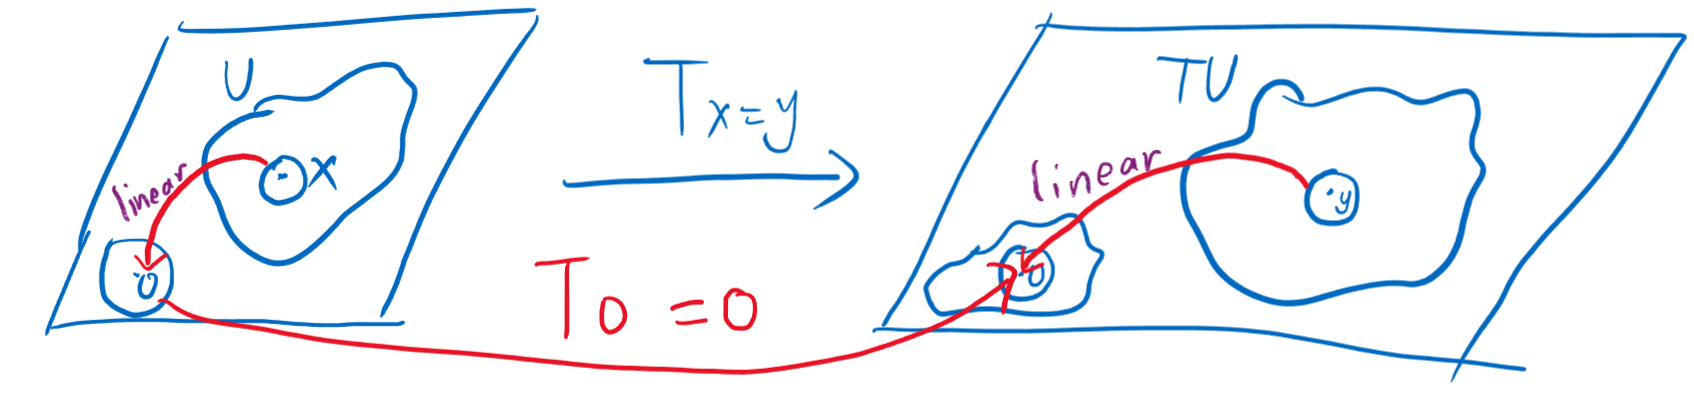
\includegraphics[scale=0.3]{./fig/4.4-1.png}
\end{figure}

\textbf{Proof}:分两步证明$T0$是$TB(0,1)$的内点。

\textbf{Step 1. }证明$T\overline{B(0,1)}$在某个$B_1(0,\delta)$中稠密。

由于$T$是满射,即$TX=X_1$,且$X_1$是全空间
\[X=\bigcup_{k=1}^{\infty}\overline{B(0,k)} \quad \Rightarrow \quad X_1 \subseteq \bigcup_{k=1}^{\infty}T\overline{B(0,k)} \quad \Rightarrow \quad X_1=\bigcup_{k=1}^{\infty}T\overline{B(0,k)}\]

由于$X_1$是$Banach$空间,为第二纲集,故存在某个开球$B_1(y_0,r_0) \subset T\overline{B(0,K_0)}$。
\[\forall y \in B_1(0,r_1) \ , \ y=\frac{1}{2}[(y_0+y)-(y_0-y)]:=\frac{1}{2}(y_1-y_2) \ , \ y_1,y_2 \in B_1(y_0,r_0)\]
\[\forall \varepsilon>0 \ , \ y_1,y_2 \in B_1(y_0,r_0) \ , \ \exists \, x_1,x_2 \in \overline{B(0,k_0)} \quad \text{s.t.} \quad ||Tx_1-y_1||<\varepsilon \ , \ ||Tx_2-y_2||<\varepsilon\]
\[\forall \varepsilon>0 \ , \ y=\frac{y_1-y_2}{2} \in B_1(0,r_1) \ , \ \exists \, x=\frac{x_1-x_2}{2} \in \overline{B(0,k_0)} \quad \text{s.t.} \quad ||Tx-y||=\left\|T\left(\frac{x_1-x_2}{2}\right)-\frac{1}{2}(y_1-y_2)\right\|<\varepsilon\]
即$T\overline{B(0,k_0)}$在$B_1(0,r_0)$中稠密,从而$\forall \varepsilon>0 \ , \ T\overline{B(0,\varepsilon)}$在$B_1(0,\delta\varepsilon)$中稠密,其中$\delta=r_0/k_0$,可取$\varepsilon=1$。

\textbf{Step 2. }证明$T\overline{B(0,1)} \supset B_1(0,\delta/2)$。

由$T\overline{B(0,1/2)}$在$B_1(0,\delta/2)$中稠密,可知
\[\forall y \in B_1(0,\frac{\delta}{2}) \ , \ \exists \, x_1 \in B(0,\frac{1}{2}) \quad \text{s.t.} \quad ||y-Tx_1||<\frac{\delta}{2^2} \quad \Leftrightarrow \quad y_1:=y-Tx_1 \in B_1(0,\frac{\delta}{2^2})\]
以此类推可得
\[\exists \, \{x_n\} \subset B(0,1) \ , \ ||x_n|| \leq \frac{1}{x^n} \ , \ \left\|y-T\left(\sum_{k=1}^nx_k\right)\right\|<\frac{\delta}{2^{n+1}}\]
\[S_n:=\sum_{k=1}^nx_k \ , \ m>n>N \ , \ ||S_m-S_n||=\left\|\sum_{k=n+1}^mx_k\right\| \leq \sum_{k=n+1}^m||x_k||<\frac{1}{2^{n+1}} \to 0\]
$\{S_n\}$是$Cauchy$列,在完备空间$X$中收敛,记为$S$,则
\[||y-TS||=\left\|y-T\lim_{n \to +\infty}\sum_{k=1}^nx_k\right\| \leq \lim_{n \to +\infty}\left\|y-T\sum_{k=1}^nx_k\right\|=0\]
命题即证。

综上所述,有
\[TB(0,1) \supset T\overline{B(0,\frac{1}{2})} \supset B_1(0,\frac{\delta}{4})\]

即对$x=0 \in B(0,1)$我们能找到$y=Tx=0 \in TB(0,1)$是$TB(0,1)$内点。结合之前的分析,定理得证。

\textbf{Q.E.D.}

完成上面这么一个大工程,我们现在终于能回答一开提及的关于逆算子性质的问题了。
\begin{theorem}[逆算子定理]
    设$X,X_1$是$Banach$空间,$T \in \mathscr{B}(X,X_1)$是一一映射(保证开映射),$TX=X_1$,则$T^{-1} \in \mathscr{B}(X_1,X)$。
\end{theorem} 
\textbf{Proof}:由开映射定理中的Step 2可知
\[T\overline{B(0,1)} \supset B_1(0,\frac{\delta}{2}) \quad \Rightarrow \quad \forall z \in X_1 \ , \  \frac{z\delta}{4||z||} \in B_1(0,\frac{\delta}{2}) \ , \ \exists ! \, T^{-1}\left(\frac{z\delta}{4||z||}\right) \in \overline{B(0,1)}\]
\[\left\|T^{-1}\left(\frac{z\delta}{4||z||}\right)\right\| \leq ||T^{-1}|| \cdot \left\|\frac{z\delta}{4||z||}\right\| \leq 1 \quad \Rightarrow \quad \frac{||T^{-1}z||}{||z||} \leq \frac{4}{\delta} \quad \Rightarrow \quad ||T^{-1}|| \leq \frac{4}{\delta}\]

\textbf{Q.E.D.}

由逆算子定理我们还有个推论。
\begin{proposition}
    若线性空间$X$上有两个范数$||\cdot||_1,||\cdot||_2$,使得$(X,||\cdot||_1),(X,||\cdot||_2)$都是$Banach$空间,且$||\cdot||_1$强于$||\cdot||_2$,则$||\cdot||_1$与$||\cdot||_2$等价。
\end{proposition}
\textbf{Proof}:定义映射$I:(X,||\cdot||_1) \to (X,||\cdot||_2) \ , \ x \mapsto x$。
显然$I$是可逆算子,且由$||Ix||_2=||x||_2 \leq \alpha ||x||_1$可知$I$有界。
由逆算子定理,$I^{-1}:(X,||\cdot||_2) \to (X,||\cdot||_1) \ , \ x \mapsto x$,有$||Ix||_1=||x||_1 \leq \beta ||x||_2$,原命题得证。

\textbf{Q.E.D.}

本小结最后我们将介绍闭图像定理,首先先定义一下什么是图像。
\begin{definition}[图像,闭图像]
    设$T:X \to Y$是映射,称$G(T)=\{(x,Tx)|x \in X \times Y\}:=\{(x,Tx)|x \in X ,y \in Y\}$为$T$的图像。\\
    若$G(T)$是$X \times Y$中的闭集,则称$T$为闭算子,即
    \[\forall \{(x_n,y_n)\} \subset G(T) \ , \ x_n \to x \in X \ , \ y_n \to y \in Y \ , \ (x,y) \in G(T)\]
\end{definition}
\begin{theorem}[闭图像定理]
    设$X,Y$是$Banach$空间,若$T:X \to Y$是闭线性算子且$D(T)$是比线性子空间,则$T$是有界的。
\end{theorem} 
\textbf{Proof}:由于$T$是闭算子,故$G(T)=\{(x,Tx)|x \in D(T)\}$是$X \times Y$的闭线性子空间,从而$G(T)$是$Banach$空间,考虑算子$p:G(T) \to D(T) \ , \ (x,Tx) \mapsto x$,易知$p$良定义且为一一映射,且满足线性,且$p$有界
\[||p(x,Tx)||=||x||_X \leq ||(x,Tx)||_{X \times Y} \leq ||x||_X + ||Tx||_Y\]
由逆算子定理$\exists \, p^{-1}:D(T) \to G(T) \ , \ x \mapsto (x,Tx)$有界,即
\[||p^{-1}x||=||(x,Tx)||_{X \times Y}=||x||_X + ||Tx||_Y \leq \alpha ||x||_X \quad \Rightarrow \quad ||Tx||_Y \leq \beta ||x||_X\]

\textbf{Q.E.D.}

考虑$X,Y$是$Banach$空间,$T \in \mathscr{B}(X,Y)$,如果$D(T)$是闭的,则$G(T)$是闭的
\[\forall\{(x_n,y_n)\} \subset G(T) \ , \ x_n \to x \in D(T) \ , \ y_n=Tx_n \to Tx=y \in T(D(T)) \quad \Rightarrow \quad (x,y) \in G(T)\]
若$D(T)$不是闭的,可以考虑如下延拓
\[x_n \to x \in \overline{D(T)} \ , \ \overline{T}:\overline{D(T)} \to Y \ , \ x \mapsto T\overline{x}=\lim_{n \to \infty}Tx_n\]

一般来说闭算子不一定有界($X,Y$是$Banach$空间),因为$D(T)$不一定是闭子空间,如
\[X=C[0,1] \ , \ T=\dv{t} \ , \ D(T)=C^1[0,1]\]
这里,$D(T)$不是闭的,$T$是闭算子,设$x_n \to x \ , \ y_n=Tx_n=x_n' \to y$,则:
\[x_n(t)-x_n(0)=\int_0^tx_n'(s) \dd s \quad \Rightarrow \quad x(t)-x(0)=\int_0^ty(s) \dd s\]
即,$D(T)$中任意收敛于自身的点列在$T(D(T))$中也收敛于自身,但是$T$不为有界算子,因为存在反例如
\[\lim_{n \to \infty}T(\sin nx)=+\infty\]